\documentclass[11pt]{beamer}
\usepackage[utf8]{vietnam}
\usepackage{lmodern}
\usetheme{Warsaw}
\usepackage[backend=biber]{biblatex}

\addbibresource{presentation.bib}

\begin{document}
\author{Trần Hoàng Quân, Lê Hoàng Trọng Tín, Lê Mai Nguyên Thảo}
\title{Trust Negotiations}
\subtitle{Khái niệm và một số frameworks trên thực tế}
\logo{
\includegraphics[scale=.2]{img/fithcmuslogo.png}}
\institute{Trường Đại học Khoa học tự nhiên - ĐHQG HCM \\ Khoa Công nghệ Thông tin}
%\date{}
%\setbeamercovered{transparent}
%\setbeamertemplate{navigation symbols}{}
\begin{frame}[plain]
\maketitle
\end{frame}

\begin{frame}
\frametitle{Nội dung}
\tableofcontents
\end{frame}

\section{Giới thiệu}
\begin{frame}
\frametitle{Giới thiệu}
Một ví dụ trong thế giới thực: Bạn đi siêu thị mua hàng và thanh toán bằng thẻ tín dụng.
\begin{enumerate}
\item Nhân viên thu ngân xác nhận thẻ của bạn là thẻ hợp lẹ (e.g kiểm tra format số thẻ, kiểm tra 4 số security code, kiểm tra thẻ có bị chỉnh sửa tẩy xóa, ..etc).
\item Nhân viên thu ngân yêu cầu chủ thẻ nhập PIN và nhập số tiền.
\item Nhân viên thu ngân in biên lai và đưa bạn kí.
\item Nhân viên xác nhận chữ kí của bạn giống chữ kí phía sau thẻ, vậy là đã thanh toán thành công.
\end{enumerate}
\end{frame}

\begin{frame}
\frametitle{Giới thiệu (cont.)}
Giao dịch trong ví dụ trên có sự trao đổi thông tin (credentials) giữa người mua và người bán, từ đó thiết lập sự tin tưởng rằng người mua có đủ điều kiện để mua đồ, và người bán có đủ điều kiện để bán.

Mục đích cuối cùng của Trust Negotiation:
\begin{itemize}
\item Thiết lập sự tin cậy (Trust Establishment) giữa các bên tham gia.
\item Dù trao đổi nhiều thông tin (credentials) với nhau, các thông tin này phải được giữ an toàn.
\end{itemize}
\end{frame}

\section{Trust Negotiation}
\begin{frame}
\frametitle{Trust Establishment}
Trust Establishment: thiết lập sự tin cậy giữa những "người lạ" trong hệ thống mở:
\begin{itemize}
\item Client và Server không cùng security domain.
\item Quyết định cấp quyền truy cập dựa vào thuộc tính (attribute), không dựa vào danh tính (identity).
\begin{itemize}
\item E.g: Quyền của client trong tổ chức, loại ngành nghề, chức vụ, ..etc
\end{itemize}
\end{itemize}
\end{frame}

\begin{frame}
\frametitle{Trust Negotiation}
Trust Negotiation: phuơng pháp tiếp cận bằng cách kiểm soát truy cập và xác thực, cho phép người yêu cầu tài nguyên (resource requesters) và nhà cung cấp (providers) thiết lập sự tin cậy trong các hệ thống mở, dựa trên các thuộc tính (attributes) hơn là danh tính (identity).
\begin{itemize}
\item Trao đổi digital credentials giữa các bên một cách tuần tự.
\item Đầu tiên trao đổi credentials ít nhạy cảm, khi độ tin cậy tăng thì trao đổi credentials nhạy cảm hơn.
\end{itemize}
\end{frame}


\begin{frame}
\frametitle{Trust Negotiation (cont.)}
\begin{figure}[H]
\centering
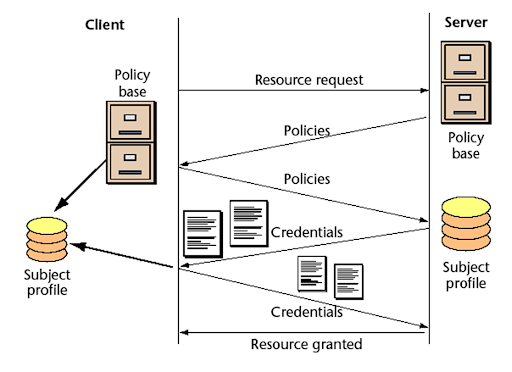
\includegraphics[scale=.4]{img/trust-simple.png}
\caption{Sơ đồ (đơn giản) của một mô hình Trust Negotiation}
\end{figure}
\end{frame}

\begin{frame}
\frametitle{Trust Negotiation (cont.) - Digital Credentials}
Digital Credentials: chứa các thuộc tính thông tin của người sớ hữu, được cấp bởi một bên đáng tin cậy (thường là nhà cung cấp chứng thư số).
\begin{itemize}
\item Khó làm giả.
\item Dễ xác thực.
\item Ký bằng khóa PKI (public-key infrastructure, e.g chuẩn X.509 v3)
\end{itemize}
\end{frame}

\begin{frame}
\frametitle{Trust Negotiation (cont.) - Credential disclosure}
Credential disclosure policy (CDP):
\begin{itemize}
\item Điều kiện để một bên công bố credentials.
\item Bản thân credentials có thể có một số yếu tố nhạy cảm, nên được xem như một tài nguyên được bảo vệ.
\item Bản thân CDP cũng là một đối tượng được bảo vệ.
\end{itemize}
\end{frame}

\begin{frame}
\frametitle{Trust Negotiation (cont.) - Requirements}
Các yếu tố cần thiết cho một hệ thống Trust Management:
\begin{itemize}
\item Quyền sở hữu đối với credential.
\item Tính hợp lệ của credential.
\item Cơ chế bảo vệ quyền riêng tư.
\item Hỗ trợ các chiến thuật thương lượng thay thế.
\item Các chiến thuật thương lượng nhanh.
\end{itemize}
\end{frame}

\section{Một số frameworks trên thực tế}
\begin{frame}
\frametitle{Trust Negotiation (cont.)}
Một số hệ thống trên thực tế:
\begin{itemize}
\item Keynote trust management system
\item Trust Establishment phát triển bởi Haifa Research lab
\item Trust Builder
\item Unipro
\item Trust-X
\end{itemize}
\end{frame}

\begin{frame}
\frametitle{Một số vấn đề với Trust Negotiation}
Một số vấn đề có thể kể đến\cite{10.1007/3-540-44875-6_20}
\begin{itemize}
\item Kiến trúc% \textit{Nên sử dụng các ứng dụng thứ ba?}
\item Chiến thuật establishing trust
\item Nhận và lưu credentials
\item Khả năng mở rộng
\item Tấn công
\item Xác thực nhiều đối tượng
\end{itemize}
\end{frame}

\begin{frame}
\frametitle{Tài liệu}
\printbibliography
\end{frame}
\end{document}